%%MAIN: thesis.tex

%%%%% The Validation %%%%%
\chapter{Implementation: Lesson Plans} \label{ch_teaching}

In its current form, the ``Processing Abstractions'' environment as presented in chapter \ref{ch_pa} is mainly targetted at the obligatory introduction to computer sciences at high school level.

Before going into empirical results from using this environment in two courses, three lesson plans will be presented for which it has been developed: a \emph{Sichtenwechsel} in computer architecture (section \ref{sc_lesson_ca}); an introduction into the inner workings of a compiler (section \ref{sc_lesson_compiler}); and first a plan for a general introduction to programming (section \ref{sc_lesson_intro}). Some ideas for how to expand it for other school levels will be presented in section \ref{sc_lesson_other}.

For all the lessons, students will need a local environment of ``Processing Abstractions'' installed on a computer available to them. See appendix \ref{app_setup} for how to set it up. Additionally, for non-German speaking students the contents will have to be translated to the teaching language.



\section{Introduction to Programming} \label{sc_lesson_intro}

While the ``Processing Abstractions'' environment has been developed for linking programming and computer architecture, it can also be used for an introduction to programming. This does even help linking programming and computer architecture for students, since they can start at the same point and reuse the experience already gained.


\subsection{Educational objective}

After the introduction, students should be able to \dots
\begin{itemize}
\item work within GT.
\item read, write and understand programs with a limited command set, including working with the implicit animation loop.
\item learn from their mistakes, correct themselves and not be afraid of breaking things.
\end{itemize}

In the end, students should have a solid foundation for taking on the task of writing a basic but still interesting app or game.\footnote{Possible ideas, which all have been implemented by students, include: ``Flappy Bird'', ``Geometry Dash'', ``Pong'', ``Doodle Jump'', ``Snake'', a quiz, a labyrinth, \emph{etc.}. For most of these, ``Processing Abstractions'' provides sufficent support, the main deficit being the lack of keyboard input.}


\subsection{Prerequisites}

Students need experience in using their own computer, including \dots
\begin{itemize}
\item downloading and extracting archives, and
\item dealing with their virus scanner.\footnote{At least under Windows, many scanners flag GT as untrustworthy due to its executable lacking a valid signature. Some virus scanners even block the entire download, if the archive is distributed over a network.}
\end{itemize}

Additionally, the teacher must prepare their contents in GT e.\,g. as described in \ref{app_setup} and distribute them. Ensure that the first lesson page will be displayed on first startup.


\subsection{Introduction to Glamorous Toolkit} \label{ssc_lesson_gt}

Since Glamorous Toolkit will be a new environment altogether for all students, some basics on its usage have to be introduced first within ten minutes:

\begin{instructions}
\item Ask students to download and extract your GT distribution as homework for the first lesson. Under Windows, they might run into a first issue with their virus scanner blocking the download, so remind them about what to do in that case.\footnote{In most virus scanner settings, the warning can be overruled by the user; else they might have to \emph{temporarily} disable scanning for this one download.}
\item Tell students to start GT and open the notebook page about working with Glamorous Toolkit (``Arbeiten mit Glamorous Toolkit'' in the included teaching materials). Also ask them to help their neighbours, if they see them struggling. Use the time while students are reading and doing the first tasks for ensuring that everyone has managed to get GT running.
\item Introduce GT as an interactive notebook similar to what students already know from class.\footnote{Many schools have standardized on working with the Microsoft 365 Office Suite which includes OneNote.} One main difference will be that additional views will open to the side, hiding the table of contents. So show them, how to get back by selecting the left-most view (through the blue dots at the center top) and expand it (through the \faPlusCircle\ at the top left).
\item If you want students to be able to take notes of their own inside GT notebooks, show them how to move a page to their local knowledge base (where it can be backed up individually) and how to create and structure new paragraphs (\ct{Ctrl+Enter}, \ct{Alt+Shift+Arrow}). Markdown syntax for formatting does not have to be introduced explicitly, that can be replicated by students by inspecting your content.
\item Finally, keep in mind GT's ability to be inspected at every level and point more advanced students towards using these (e.\,g. by \ct{Ctrl+Shift+Alt+Click} anywhere, by double-clicking on list items, or by going through the different views of an object).
\end{instructions}

Please note that as described in \ref{sc_gt}, GT is bleeding edge technology and might not always behave the way you and your students have become used to: Since notebook pages are rendered progressively, scrolling won't always work smoothly (and will scroll inner content, if the mouse cursor isn't positioned at a page's border); occasionally unexpected error messages trigger the debugger to pop up which has to be closed again; and sometimes the keyboard modifiers may get stuck, resulting in shortcuts no longer working (which is resolved by switching to a different app and back).


\subsection{Lesson Plan}

Since this isn't the focus of this thesis, we won't go into much detail about introducing programming, but just summarize what might work within the provided environment:

Start top down as suggested in \ref{ssc_top_down} from either abstract art or games\footnote{Most one-tap games should work, e.\,g. \url{https://www.lessmilk.com/almost-pong/} has reasonably simple gameplay with minimalist visuals.} and start dissecting how this concrete entity might be described, first in natural language and then in formalized language.

Then follow Reas and Fry \cite{Rea14} and introduce the Processing language (see \ref{sc_processing}), by starting with a sequence of statements with few commands (e.\,g. \ct{size}, \ct{rect}, \ct{ellipse} and \ct{fill}), and then sequentially introducing comments, colors, variables and arithmetic, the animation loop, conditions and interactivity.

Every concept can be described on a notebook page with given examples for first exploring the effects of a command and its arguments\footnote{Students may either describe the expected behavior and then verify that their expectation matches the outcome, or less taxingly try given or random values and then describe their observations. Variations consist e.\,g. in a student describing desired behavior and then (another student) trying to achieve this.} and then later using the concept for solving problems by starting from a skeleton program (see figure \ref{fig_screenshot_introduction} for an example of both).

\begin{cfigure}[fig_screenshot_introduction]{Excerpt from an interactive notebook page with exploratory and live programming tasks.}
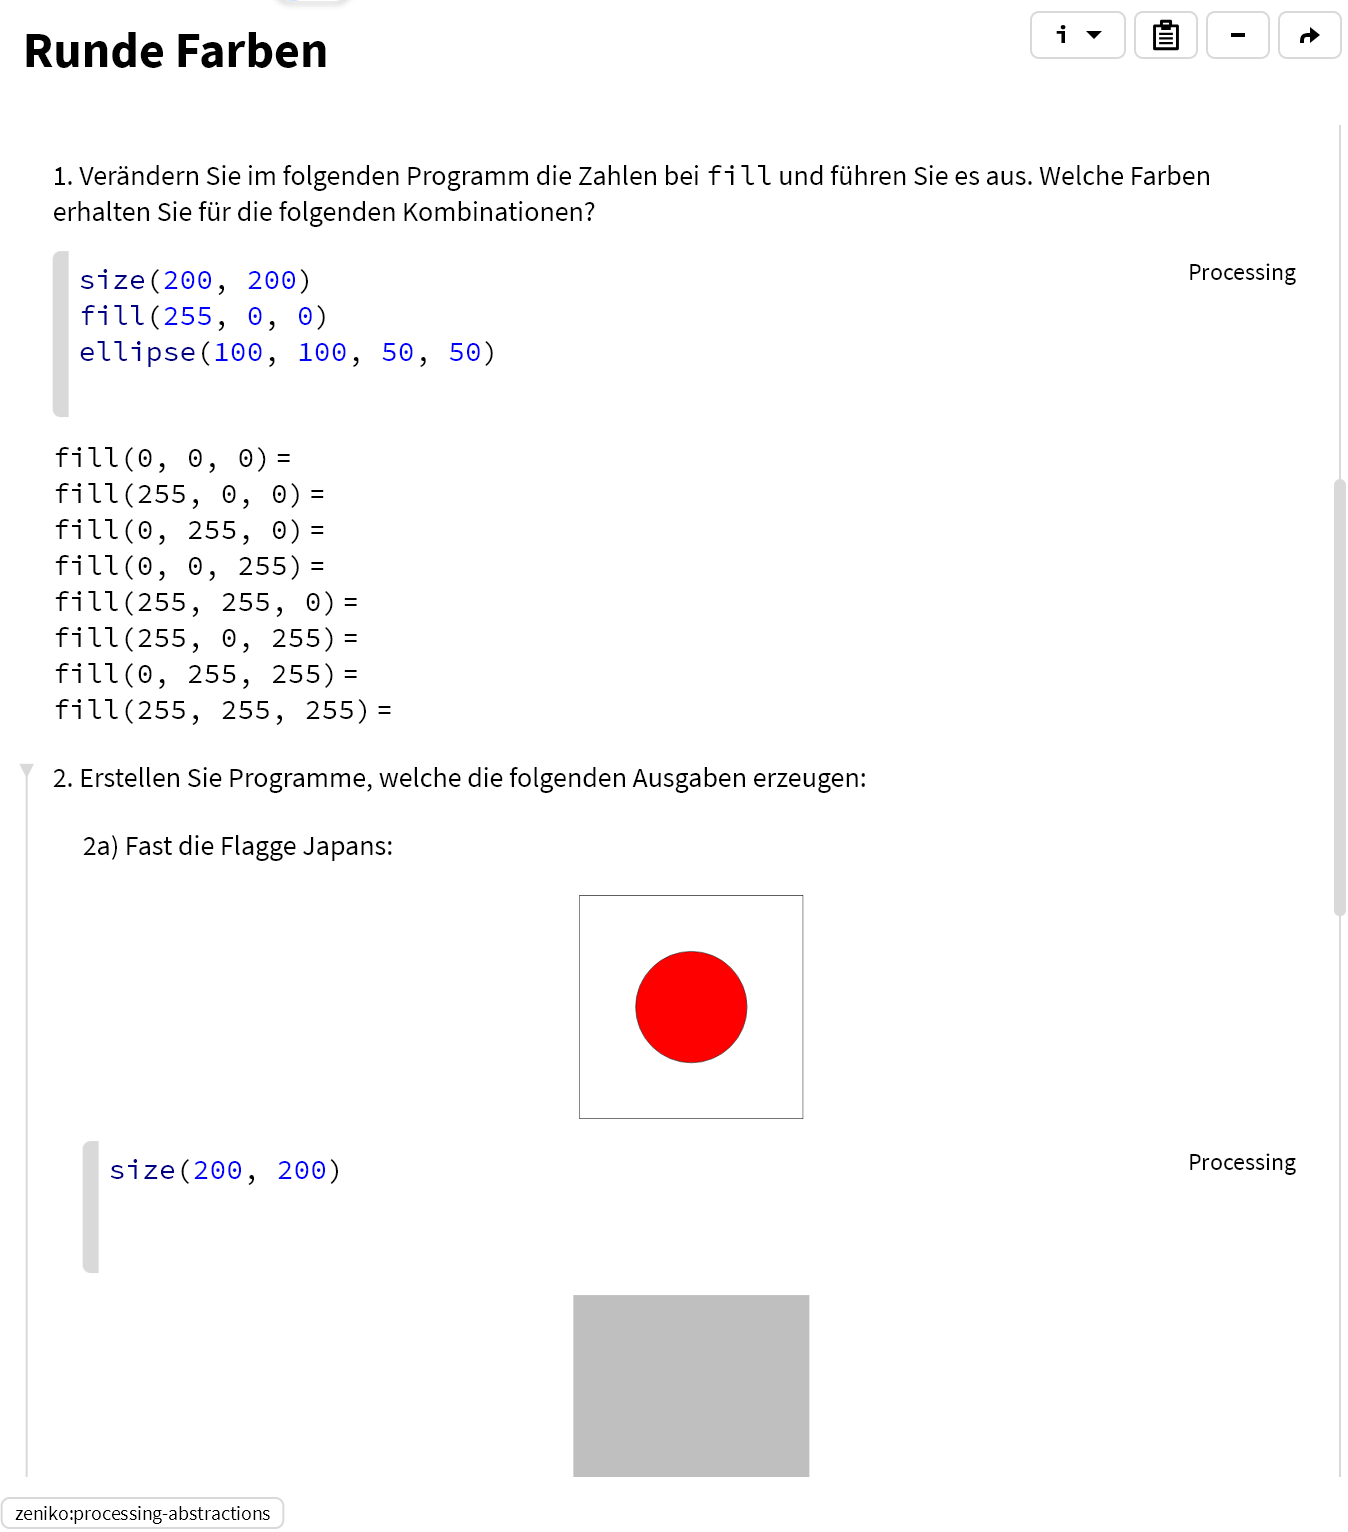
\includegraphics[width=.7\textwidth]{screenshot_introduction}
\end{cfigure}

At the beginning, debugging will only consist in modifying values and observing live changes until the desired output is reached. At later stages, the step-by-step execution views will be useful, where executed expression, variable values and visual output are displayed side-by-side and execution can be played forward and also in reverse.

Quicker and more proficient students could also already at this point start to delve deeper: The third and fourth execution icons will lead them to discover by themselves what lies under the hood.

Sample content for this is included in the \emph{Unterrichtsmaterialien} of  ``Processing Abstractions'' as ``\emph{Programmieren mit Processing}''.



\section{Lesson on Computer Architecture} \label{sc_lesson_ca}

The main objective of this thesis was to demonstrate, how understanding of what happens when executing a program could be improved by having students perform a \emph{Sichtenwechsel}. The same goes for the other way around, where computer architecture is explained in more concrete form by tying it to previous programming experience.

Introductions to computer science which extend beyond a pure programming course often contain lessons on computer architecture. E.\,g. the curriculum \cite[p.\,145]{Erz16} asks for students to ``know how computers and networks are structured and work''.

We again propose to approach this task top down (see \ref{ssc_top_down}) and move along the path specified in figure \ref{fig_multitier}. This will be outlined here with validation of part of this approach following in \ref{sc_validation_ca}.

With respect to manageability (see \ref{ssc_manageability}), it is proposed to mostly skip the inner workings of a compiler and treat that in a separate sequence (maybe only for students specializing in computer science).


\subsection{Educational objective}

After these lessons, students should be able to \dots
\begin{itemize}
\item explain the concepts of (virtual) machine, memory, stack, machine language, and program counter (with relation to a von Neumann model).
\item elaborate why machine language must be different from a high-level language such as Processing.
\item explain why some commands are slower than others.
\item connect their knowledge about encodings with how values and machine code are stored.
\item consequently understand how one of their programs might be run on actual hardware and document their understanding with correct terms.
\end{itemize}


\subsection{Prerequisites}

Students must already have basic programming skills in a high level language. In particular, they must know about variables and loops. If they don't know Processing or at least Python yet, a brief introduction (maybe along the ideas proposed in \ref{sc_lesson_intro} above) is required.


\subsection{Lesson Plan}

Whereas Nisan and Schocken \cite{Nis21} introduce their bottom up course with a top down overview, we propose doing the same in reverse for this top down approach:

\begin{instructions}
\item Start with a brief repetition on programming by giving students a few quickly solved tasks (including one about the animation loop, where at least the skeleton structure is given). If this is the student's first encounter with Glamorous Toolkit, use this opportunity to introduce it (see \ref{ssc_lesson_gt}).
\item Show students the innards of a computer and ask where their programs reside in there. Use this for discussing hard drives and volatile memory, and a repetition about encodings and how everything boils down to \texttt{1}s and \texttt{0}s (or current and no current respectively).
\item Briefly start at the desired lowest abstraction layer, e.\,g. (light) switches, and explain how they're used for creating processors.
\item Ask students about games they play and have them describe possible player \emph{actions} and compare them with actual player \emph{input}.\footnote{Alternatively, if starting from art instead of games, decompose drawing e.\,g. a house into individual brush strokes}. This repeats top down abstraction decomposition as maybe already encountered in the introduction to programming lessons and allows to bring the foundational idea of multitier architectures back to students minds.\footnote{Multitier architectures might already have been discussed as part of networking lessons.}
\item Have students go back to a sample or one of their own Processing progams and let it (again) be displayed in machine code. Provide them several examples, e.\,g. with variable assignment, with conditionals and loops, and let them assemble the required machine code mnemonics and byte values.\footnote{Ideally, distribute the examples over small student groups, two groups per example.} Suggest variations for the example, so that even with less programming experience they may find regularities.
\item Collect their findings and group their arguments: pushing to the stack/accumulator (machine codes 0--83), returning (88--94), binary arithmetic and comparison operations (96--111), common commands (112--127), message sending/function calls (128--175), jumps (176--199), storing results (200--216), combined multi-byte instructions (first byte: 224--255) \cite[p.\,12]{Ber14}.\footnote{Students should at this point be able to explain where these seemingly odd number ranges stem from.}
\item Take a step back: What is relevant for running a program? This should yield memory, (arithmetic) operations, input and output and control flow. Let students go back to their examples and see if Processing code doing for one or multiple of these core concepts map to the found machine codes.
\item Introduce von Neumann architecture (see figure \ref{fig_von_neumann}) as an abstraction of the encountered concepts. What physical parts of a computer belong to the idealized concepts?
\item Discuss virtual machines in comparison to physical machines\footnote{VMs being used for portability reasons such as the Smalltalk VM, the Java VM, Microsoft's dotNet VM or any browser's VM for WASM.} and the difference of stack and register machines, VMs tending to the former and physical machines to the latter.
\item Go back to Processing and inspect a combined execution view (see figure \ref{fig_screenshot_vm_execution}). By stepping forward and backward, students should be able to observe the role of the stack and the program counter. Let them explore execution flow and write down what role the program counter has and what the calling convention for Processing API calls seems to be.
\item As a break or maybe as homework, let students play ``Human Resource Machine''\footnote{The ``Hour of Code Edition'' is free to download for notebooks.} \cite{Tom15}, which introduces students to a different architecture. The first 6 levels should be doable for everybody, with quicker students finding sufficient challenges later on.\footnote{You can also come back during compiler lessons, as ``Human Resource Machine'' has implementing various optimizations as additional challenges.}
\item Compare the two instruction architectures with relation to expressitivity and register vs. stack based design.

\item Finally, treat circuits, logic gates, transistors and maybe down to silicon outside of GT to the desired depth.
\end{instructions}

\begin{cfigure}[fig_von_neumann]{Von Neumann architecture.}
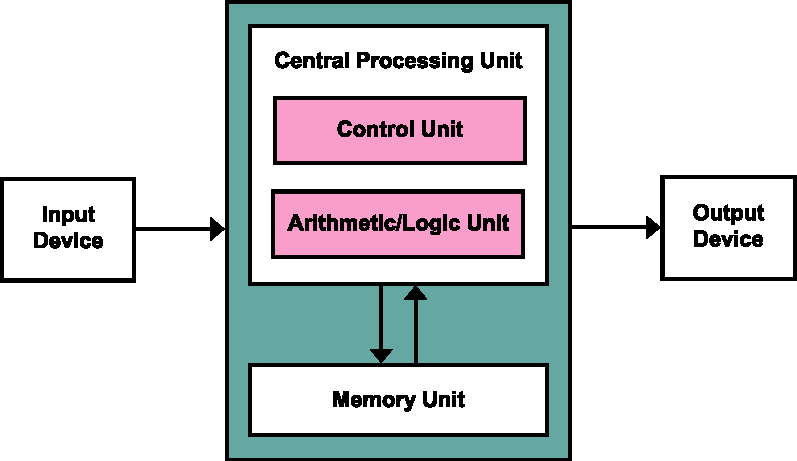
\includegraphics[width=10cm]{Von_Neumann_Architecture}
\begin{todo}
\item replace or properly attribute: Kapooht, 2013, CC BY-SA 3.0
\end{todo}
\end{cfigure}

\begin{cfigure}[fig_screenshot_vm_execution]{Excerpt from an interactive notebook page on program execution in a VM.}
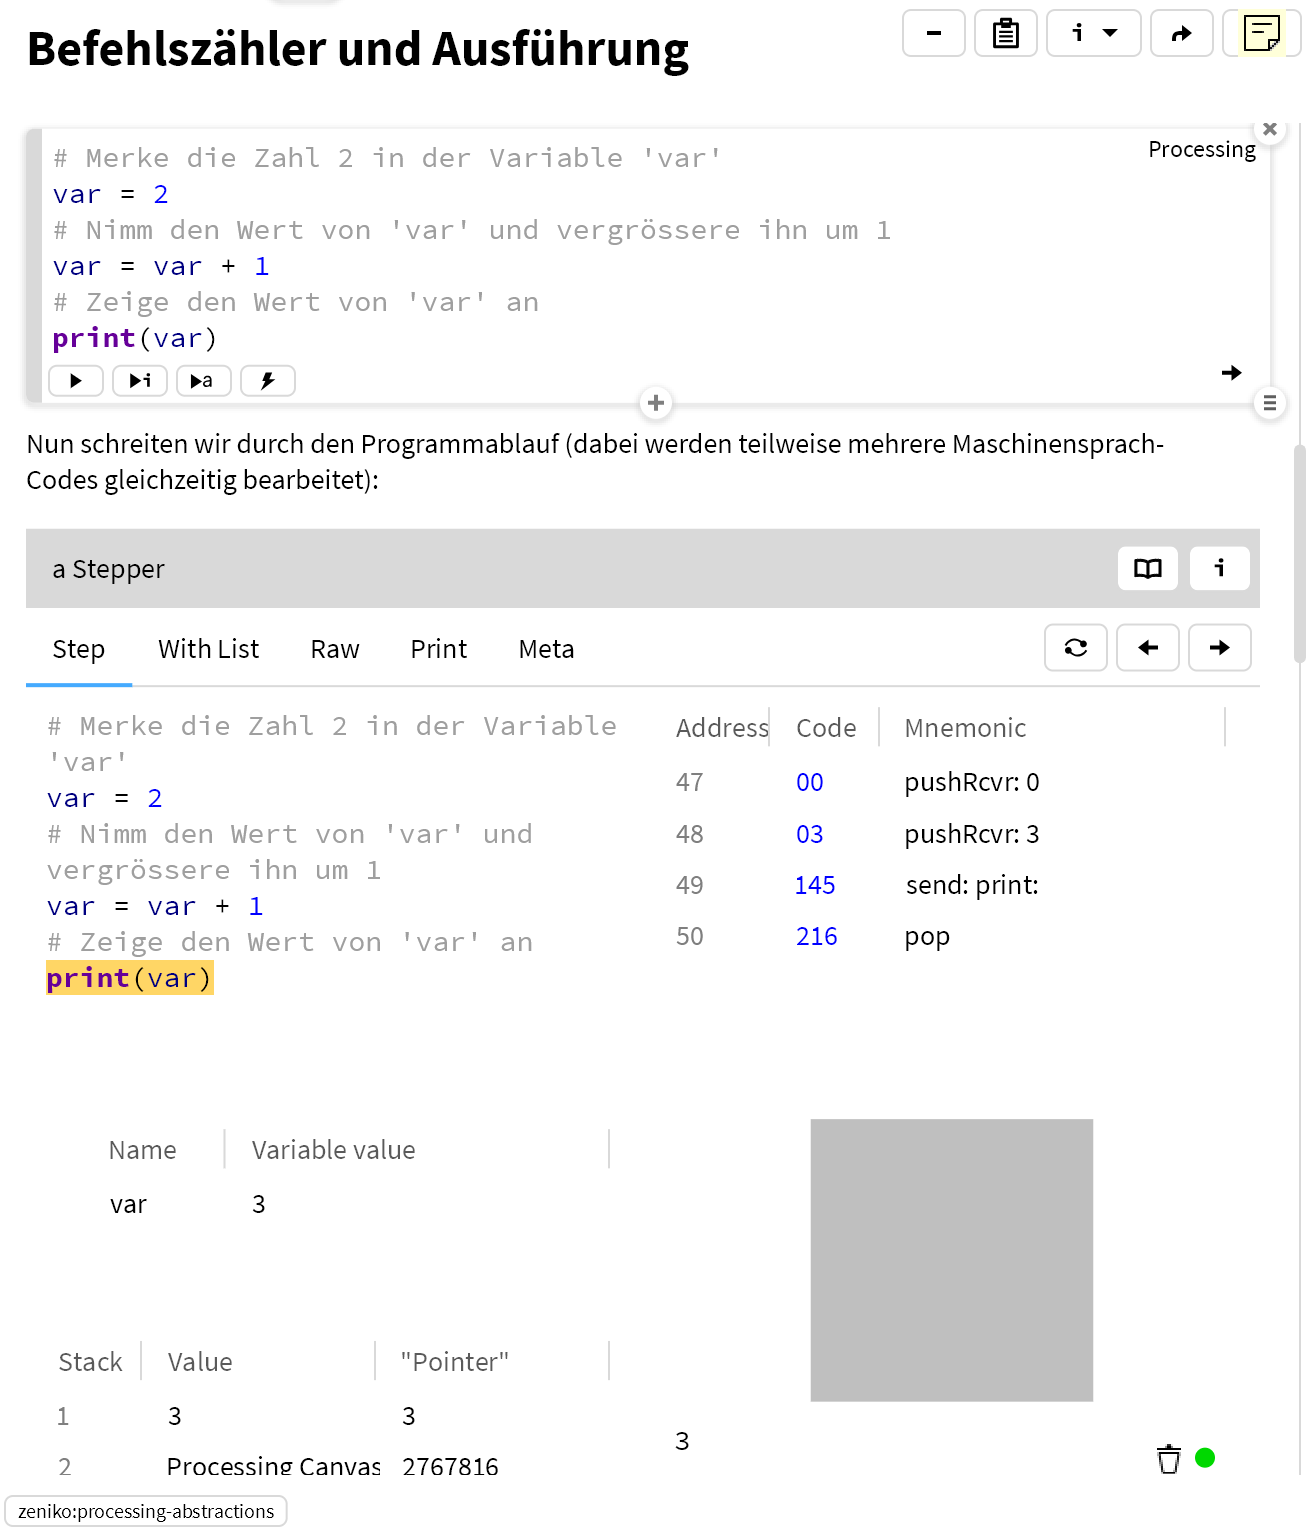
\includegraphics[width=.7\textwidth]{screenshot_vm_execution}
\begin{todo}
\item Decide which screenshots belong into the appendix instead.
\end{todo}
\end{cfigure}



\section{Lesson on Compilers} \label{sc_lesson_compiler}

Once students have an approximate understanding of into what a program must be transformed in order to be run on actual hardware or inside a VM, the question remains as to how the transformation from source code to machine code happens.

While this is usually not in the focus of a general introduction into computer science beyond the superficial treatment occurring during the lessons on computer architecture, this is quite relevant for students specializing in computer science.

However, using the environment presented here, this topic could just as well be used either for all students or for quicker students to work on mostly by themselves. Part of the lesson presented here has indeed been validated under these circumstances (cf. \ref{sc_validation_compiler}).


\subsection{Educational objective}

After these lessons, students should be able to \dots
\begin{itemize}
\item explain the difference between high and low level languages.
\item enumerate the steps required during compilation, using proper terminology (lexer, parser, transpiler, compiler, optimizer).
\item connect this knowledge with their knowledge on computer architecture and programming.
\end{itemize}


\subsection{Prerequisites}

Students must have experience in programming and computer architecture, e.\,g. from the lessons described above (cf. \ref{sc_lesson_introduction} and \ref{sc_lesson_ca}). It helps, if their programming experience is based on Processing or at least Python. Additionally, the need to have GT installed and introduced (see \ref{ssc_lesson_gt}).


\subsection{Lesson Plan}

The natural way to progress on understanding a compiler is top down, which is the same as chronological order:

\begin{instructions}
\item Before starting to fill in the content missing from the previous lesson on computer architecture, begin with a repetition on how a program is run in a VM (see figure \ref{fig_screenshot_vm_execution}), letting students run again a given or one of their own program and seeing into what commands their code was translated.
\item As an analogy, analyse with students how they would go about translating an unknown language using just a dictionary: splitting the text into words where punctuation yields some structure; then looking words up (where again several words might belong together for the sake of translation\footnote{Compare e.\,g. the meanings of ``see'', ``see to'', ``see through'' and ``see out''.}); writing the translation down; and finally rewriting it so that it sounds more akin to how you'd write it in the target language. This analogy yields a fitting overview over the different steps involved.
\item Now let students work through discovering the individual concepts encountered:
\begin{itemize}
\item Have them compare a program and the resulting lexed tokens: What modifications to a program result in different tokens, what modifications don't cause changes? What does this correspond to in the analogy about translating a natural language?
\item Have them compare the abstract syntax trees resulting from their program(s). Are they able to explain how the parser structures the tokens together? How would they go about if all they saw were just two tokens? (For this, use a view of tokens showing just two lines.)
\item Discuss how a recursive descent parser works through tokens. Since Python and thus Processing based on Python uses indentation for command grouping, also highlight the need for tracking indentation at least per statement.
\item Optionally have students compare given Processing source code with the resulting AST and transpiled Smalltalk: How literal is the translation? What is different between Processing and Smalltalk? Have them try to invent a syntax of their own which is easier to map to the AST (and later discuss Lisp and Forth syntaxes as examples for alternative, easier to parse syntaxes\footnote{Views for variants of both are available.}).
\item Since usually, an intermediary representation is directly produced from an AST, collect common statement types (variable assignment, function calls, loops, \dots) and have them translated live to intermediary representation. Let students work out common patterns to see what translation might take place.
\item Have views for intermediary representation and actual Smalltalk bytecode side-by-side for students to figure out, what transformations remain and why these might be required (comparing with their knowledge from computer architecture lessons).
\item Should students have prior experience with ``Human Resource Machine'' \cite{Tom15}, have them translate Processing to a program in that game's simplified language and translate code for a level of that game back to Processing (and from that Smalltalk bytecode with the environment's help).
\item For the final step, offer some simple code examples which can obviously be simplified.\footnote{E.\,g. \ct{print(1+1+1+1+1)} or \ct{for i in rnage(10): pass}, both of which should be trivially optimizeable}. What optimizations are present in the intermediary representation and which in bytecode? What patterns could be optimized? Also discuss the difference of optimizing for size, for speed and for quick compilation.\footnote{For players of ``Human Resource Machine'', the first two are the bonus challenges for all later levels.}
\end{itemize}
\item What can't be shown inside GT are the equivalent of optimizations within a processor (or already the x86, IA64, \emph{etc.} code produced by the Just in Time compiler). Students should at this point however have sufficient understanding of the various transformations, that they might be able to understand what happened e.\,g. with the Spectre attack \cite{Koc19} and why understanding of machine code might be relevant for timing attacks.
\end{instructions}



\section{Further Lesson Ideas} \label{sc_lesson_other}

Whereas the environment presented here is mainly targeted at introductionary high school classes, it might also be employed in a specialization course. Since this isn't this thesis' focus, we'll just list a few ideas:

\begin{itemize}
\item Smalltalk is a rather elegant language and has aged quite well. It can still be used to introduce students into pure object oriented programming with a for them somewhat unusual syntax. And such an introduction could use transpilations from ``Processing Abstractions'' as a stepping stone, if students have already used it.
\item Since the here provided code is run dynamically in Glamorous Toolkit, it can also be molded further, e.\,g. to implement as of yet missing support for object oriented programming.
\item The provided code might also be used as a template for students to implement their own programming language or see if they manage to write an interpreter for one of the two provided prefix and postfix mini-languages.\footnote{This might already have been discussed in the compiler lessons above. Very briefly, a program such as \ct{a = 42; print(a)} is translated to \ct{(= a 42) (print a)} and \ct{\$a 42 = a print} respectively which both should be simple enough to parse.}
\end{itemize}
